\section{Architecture Design \& Implementation}
\subsection{Overall architecture}

\begin{figure}[htb]
\centerline{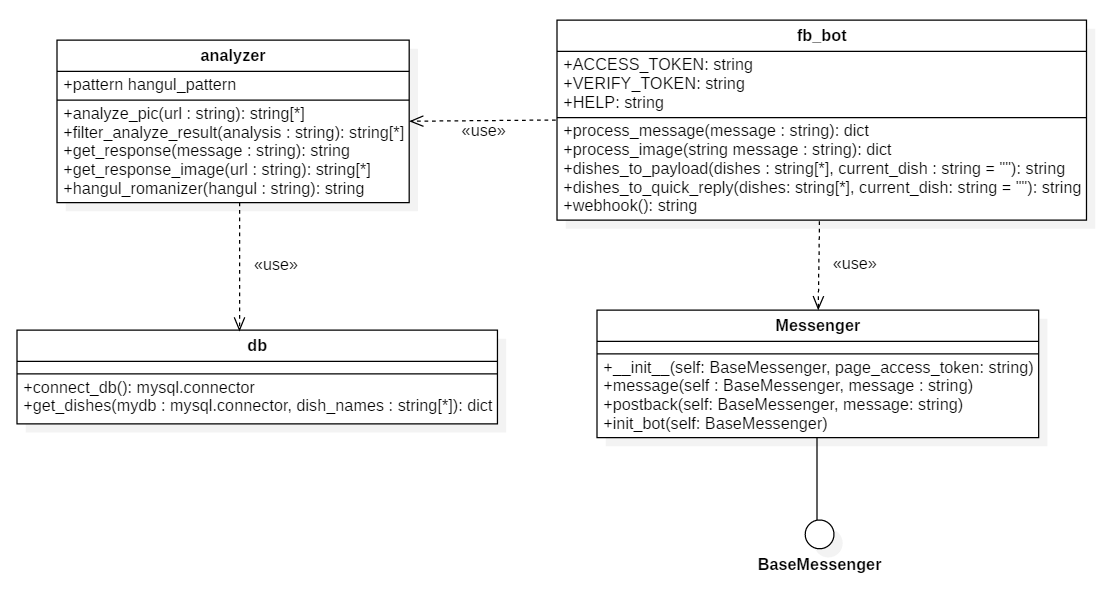
\includegraphics[width=\linewidth]{./pictures/uml}}
\caption{UML of our overall architecture}
\label{fig:uml}
\end{figure}
\FloatBarrier

\subsection{Directory organization}

\begin{table}[htbp]
\caption{Directory organization}
\begin{tabularx}{\linewidth}{|X|X|X|}
\toprule
Directory & File names & Module names in use  \\
\midrule
./src & messenger.py & messenger  \newline\\
./src & fb\_bot.py &  fb\_bot\newline \\
./src & ssl\_certificate.pem db.py \newline  & db \\
./src & analyzer.py & analyzer \newline \\
./tests & 
test.txt \newline 
test\_db.py \newline
test\_json.py	 \newline
test.jpg  \newline
& test\\
./db & food.mwb \newline & db model  \\
./doc & before\_order.tex before\_order.pdf \newline & documentation  \\
./doc/content & architecture\_design\_a nd\_implementation.tex development\_environ ment.tex introduction.tex requirements.tex specifications.tex \newline & documentation \\
./doc/pictures & 
facebook\_dish\_info.png \newline
facebook\_friends.png \newline
facebook\_meun.png \newline
facebook\_message.png \newline
facebook\_overview.png \newline
facebook\_profil.png \newline
facebook\_response.png \newline
facebook\_response\_sele ction.png	\newline
uml.png \newline
class\_uml.mdj 
& documentation \\
\end{tabularx}
\end{table}
\FloatBarrier

\subsubsection{Module 1 - messenger}
Module messenger provide connection with the facebook messenger API. 

\subsubsection{Module 2 - fb\_bot}

\subsubsection{Module 3 - analyzer}

\subsubsection{Module 4 - db}

